\documentclass[11pt]{article}
\usepackage[margin=1in]{geometry}
\usepackage[numbers]{natbib}
\usepackage{graphicx}
\usepackage{amsmath,amssymb}
\usepackage{url}
\usepackage{bm}
\usepackage{booktabs}
\usepackage{array}
\usepackage{longtable}
\usepackage[table]{xcolor}
\usepackage[T1]{fontenc}
\usepackage{lmodern}
\usepackage{textcomp}
\usepackage{pgfplots}
\pgfplotsset{compat=1.18}
\usepackage{tikz}
\usetikzlibrary{arrows.meta, decorations.pathreplacing}

\renewcommand{\topfraction}{0.9}
\renewcommand{\bottomfraction}{0.5}
\renewcommand{\textfraction}{0.07}
\renewcommand{\floatpagefraction}{0.85}

\newcommand{\papertitle}{Understanding When Poisson Log-Normal Models Outperform Penalized Poisson Regression for Microbiome Count Data}

\begin{document}

\begin{center}
{\LARGE\bfseries \papertitle\par}
\vspace{1em}
{\large Daniel Agyapong$^{1}$, Julien Chiquet$^{2}$, Jane Marks$^{3}$, Toby Dylan Hocking$^{4}$\par}
\vspace{0.5em}
{\small $^{1}$School of Informatics, Computing, and Cyber Systems, Northern Arizona University, Flagstaff, Arizona, U.S.A.\par}
{\small $^{2}$UMR MIA Paris-Saclay, Universit\'{e} Paris-Saclay, AgroParisTech, INRAE, Palaiseau, France\par}
{\small $^{3}$Department of Biological Sciences, Northern Arizona University, Flagstaff, Arizona, U.S.A.\par}
{\small $^{4}$D\'{e}partement d'informatique, Universit\'{e} de Sherbrooke, Sherbrooke, Qu\'{e}bec, Canada\par}
\vspace{0.4em}
{\small Corresponding author: \texttt{da2343@nau.edu}\par}
\end{center}
\vspace{0.8em}
\begin{abstract}
Poisson log-normal (PLN) models are widely used for microbiome count data, but prior evaluations rely on in-sample fit criteria that cannot establish whether the latent dependence structure improves generalisation over simpler penalized Poisson regression.
We introduce Leave-One-Taxon-Out cross-validation (LOTO-CV) as a held-out evaluation framework for Poisson count models and apply it to provide the first out-of-sample comparison of PLN and \texttt{GLMNet(Poisson)} on real microbiome data.
Across 20 datasets spanning $N = 32$--$18{,}270$ and $D = 24$--$257$, PLN outperforms \texttt{GLMNet(Poisson)} with gains up to 38\%, and the winner is predictable: PLN wins in 12 of 14 datasets with $N/D < 5$ and in none of the 6 with $N/D \geq 5$.
Mean absolute correlation (MAC) is the strongest secondary signal and overdispersion provides additional discriminative power.
For network inference, we evaluate PLNNetwork and \texttt{GLMNet(Poisson)} neighbourhood selection against all five publicly available datasets with experimentally validated microbial interaction truth — the complete set of such resources currently in the literature.
PLNNetwork performs best on broad undirected interaction benchmarks, whereas \texttt{GLMNet(Poisson)} is better aligned with local or directional effects.
These results give practitioners concrete, data-driven guidance for deciding when latent dependence modeling justifies its added complexity.
\end{abstract}

\noindent\textbf{Keywords:} Benchmarking; microbiome; network inference; penalized regression; Poisson log-normal.

\section{Introduction}
Microbial communities profiled by Next-Generation Sequencing produce count data with distinctive statistical properties.
Observations are nonnegative integers, contain many zeros, and are strongly overdispersed.   
Moreover, the number of taxa $D$ routinely exceeds the number of biological samples $N$~\citep{lagkouvardos2016imngs, Kodikara2022}.
These properties jointly challenge the assumptions of standard Gaussian models and limit the use of conventional Poisson regression, which cannot accommodate residual correlations among taxa or the extra-Poisson variability that arises from unobserved biological heterogeneity~\citep{mcmurdie2014waste, Chiquet2021}.

The Poisson Log-Normal (PLN) model addresses these limitations by introducing a latent Gaussian layer that captures both overdispersion and dependence among taxa within a principled probabilistic framework~\citep{aitchison1989multivariate, Chiquet2021}.
This latent structure supports a family of downstream analyses, including conditional prediction, dimensionality reduction, and the recovery of sparse ecological interaction networks through graphical lasso regularization~\citep{chiquet2019variational}.
The PLN family is fitted using variational inference and has been increasingly applied in microbiome studies that require explicit modeling of taxon dependencies~\citep{Chiquet2021, Subedi2025}.

Despite this appeal, PLN models carry a practical cost.
Estimating a full $D \times D$ latent covariance matrix scales cubically in $D$, making PLN computationally demanding for the large, sparse count tables typical of modern microbiome surveys.
By contrast, penalized Poisson regression implemented efficiently in \texttt{glmnet}~\citep{Friedman2010} fits each taxon independently using $\ell_1$ regularization, scales near-linearly in $D$, and remains tractable even when $D$ runs into the thousands.
The fundamental question motivating this work is therefore empirical.
Under what conditions does PLN's added modeling complexity translate into measurable gains over penalized Poisson regression?

This question has direct practical consequences.
A researcher analyzing a dataset with $N = 50$ samples and $D = 200$ taxa faces a genuine modeling choice between investing in PLN's joint estimation at computational cost and relying on the faster penalized regression baseline.
Existing literature provides limited guidance.
Prior evaluations of PLN variants have largely focused on illustrative case studies, synthetic data, or narrow analytical tasks, assessing goodness of fit on training data rather than held-out predictive performance~\citep{Chiquet2021, Batardiere2025ZIPLN, Chaussard2025PLNTree}.
As summarized in Table~\ref{tab:related_work}, systematic comparisons against penalized regression baselines on real microbiome data under a unified and reproducible evaluation protocol remain absent from the literature.
This gap is not merely a matter of coverage: in-sample criteria such as ELBO, BIC, and AIC measure how well a model fits the data it was trained on, not whether its latent structure captures signal that transfers to unseen observations.
A model that overfits the latent covariance can appear superior by in-sample criteria while actually performing worse out of sample.
The absence of held-out evaluation has therefore left the practical question --- when does PLN's complexity pay off? --- unanswerable from existing work.

A similar gap exists for network inference.
PLNNetwork recovers ecological interaction networks by estimating a sparse latent precision matrix~\citep{chiquet2019variational}, while neighbourhood selection through \texttt{GLMNet(Poisson)} offers an alternative route to network recovery without a joint model~\citep{Meinshausen2006, Friedman2010}.
To our knowledge, no study has evaluated these competing approaches against experimentally validated microbial interactions, which are necessary for a principled comparison of edge recovery performance.

In this paper, we address both gaps.
For count prediction, we introduce Leave-One-Taxon-Out cross-validation (LOTO-CV)~\citep{agyapong2025cross} as a held-out evaluation framework for Poisson count models.
LOTO-CV withholds each taxon in turn, predicts its counts from the remaining taxa, and scores those predictions with held-out Poisson deviance --- an out-of-sample criterion that in-sample approaches cannot provide.
We apply this protocol to compare PLN and \texttt{GLMNet(Poisson)} across 20 real microbiome datasets spanning a wide range of sample sizes and dimensionalities.
For network inference, we assemble all five publicly available datasets with experimentally validated microbial interaction truth and evaluate PLNNetwork against \texttt{GLMNet} neighbourhood selection against each.
To our knowledge, this is the complete set of such resources currently available in the literature; their scarcity reflects the difficulty of obtaining ground-truth interaction data in microbial systems.
Together, these experiments provide the first unified empirical map of when PLN's latent dependence modeling confers a genuine advantage over penalized Poisson regression.
Figure~\ref{fig:pipeline} summarizes the shift from earlier in-sample evaluation practice to the held-out count-prediction protocol used in this study.

The remainder of the paper is organized as follows.
Section~2 reviews related work and situates this study within the existing benchmark literature.
Section~3 describes the algorithms, datasets, and evaluation protocol.
Section~4 presents results for prediction and network inference.
Section~5 discusses computational scaling.
Section~6 concludes.

\section{Related Work}

Microbiome abundance data poses statistical challenges that motivate specialized count models; this section reviews the modelling choices that underlie PLN and the benchmarks that have evaluated it.
Table~\ref{tab:related_work} summarizes how prior studies approach evaluation.

\paragraph{Count data properties of microbiome surveys.}
Microbiome surveys via 16S rRNA amplicon sequencing or shotgun metagenomics produce read-count tables of non-negative integers whose observed values depend on the total number of reads sequenced per sample~\citep{HMP2012, Thompson2017, Xia2023}.
Three properties of these counts make standard Gaussian regression inappropriate. 
The latter two also show that plain Poisson regression is insufficient, motivating latent-variable extensions such as the Poisson Log-Normal.
First, \emph{compositionality}: total read depth (library size) varies across samples by orders of magnitude and carries no biological information; models that ignore this offset confound technical sequencing variation with biological signal~\citep{mcmurdie2014waste, Xia2023}.
Second, \emph{overdispersion}: counts exhibit variance far exceeding the Poisson mean, as genuine biological variation across individuals and environments inflates count variance beyond what the Poisson distribution allows~\citep{zhang2017nbmm, McCullaghNelder1989}. 
Third, \emph{excess zeros}: the majority of entries in the count matrix are zero not because taxa are truly absent but because rare taxa fall below the sequencing detection threshold, with data sparsity commonly exceeding 70\%~\citep{Batardiere2025ZIPLN, Kodikara2022}.
Gaussian regression treats counts as unbounded continuous quantities.
Ad hoc transformations such as $\log(1+x)$ can improve numerical behavior and stability, but they do not by themselves resolve discrete support or compositional structure~\citep{booeshaghi2021log1p}.

\paragraph{The Poisson Log-Normal model.}
The generalized linear model with Poisson or Negative Binomial likelihood is the natural framework for overdispersed count data~\citep{McCullaghNelder1989}.
For univariate differential abundance testing, Negative Binomial models are widely used, as implemented in DESeq2~\citep{Love2014DESeq2} and edgeR~\citep{Robinson2010edgeR}.
These are, however, marginal models: each taxon is fitted independently, so the joint dependence structure across taxa is not represented.
The Poisson Log-Normal (PLN) model, first introduced by Aitchison and Ho~\citep{aitchison1989multivariate}, addresses this by placing a multivariate Gaussian distribution on the log-intensities, capturing correlations between different taxa through a shared latent covariance matrix while still respecting the discrete, non-negative nature of the data and accommodating library-size offsets.
This makes PLN a single coherent framework for prediction, ordination, clustering, and network inference from count data~\citep{Chiquet2021, Subedi2025}.

\paragraph{Prediction and representation learning.}
Poisson PCA has been assessed primarily through simulations emphasizing principal component recovery, robustness, and computational efficiency, with microbiome datasets serving as motivating illustrations~\citep{Kenney2021PoissonPCA, Virta2023PoissonPCA}.
These studies evaluate reconstruction error and latent dimension recovery on training data rather than held-out predictive performance, and do not include penalized Poisson regression as a baseline.
The PLN framework paper \citep{Chiquet2021} presents a suite of qualitative applications spanning ordination, regression, network inference, and clustering across several ecological and microbiome datasets, but does not impose a standardized cross-validation protocol or compare against penalized regression.
Extensions addressing zero inflation and hierarchical structure compare PLN variants on synthetic and real microbiome data using in-sample criteria such as variational evidence lower bound (ELBO), log-likelihood or information criteria (AIC/BIC), and downstream discrimination or generative performance~\citep{Batardiere2025ZIPLN, Chaussard2025PLNTree}.

\paragraph{Network inference.}
Network benchmarks for count data graphical models evaluate edge recovery on synthetic PLN graphs and single-cell or gene expression data, reporting ROC curves, AUPR, and edge-weight correlations~\citep{Xiao2022PLNet}.
Synthetic data generators drawing from the PLN distribution have been developed to stress-test network algorithms under controlled graph topologies and sparsity levels~\citep{Qian2024}.
More broadly, \citet{Ghaeli2025} proposed a benchmarking framework focused on reproducibility, using bootstrap resampling to generate modified versions of real microbiome data, but stopped short of validating inferred edges against experimentally confirmed interactions.
Across these studies, edge-recovery assessment relies on synthetic or statistically constructed ground truth.

\begin{table}[htbp]
\caption{Summary of prior benchmarks of PLN and Poisson algorithms.}
\centering
\footnotesize
\setlength{\tabcolsep}{3pt}
\begin{tabular}{>{\raggedright\arraybackslash}p{2.5cm}>{\raggedright\arraybackslash}p{3.2cm}>{\raggedright\arraybackslash}p{3.2cm}>{\raggedright\arraybackslash}p{4.1cm}}
\toprule
Study (year) & Data / setting & Algorithms tested & Evaluation metrics \\
\midrule
\citet{Kenney2021PoissonPCA} & Simulations; microbiome example & Poisson PCA, PLN & Subspace recovery (principal angles); robustness to noise and exposure; runtime \\
\midrule
\citet{Chiquet2021} & Multiple ecology/microbiome case studies & PLN, PLNPCA, PLNNetwork, PLNMixture & BIC/ICL for model order selection; illustrative fits across tasks; no held-out evaluation \\
\midrule
\citet{Xiao2022PLNet} & Synthetic count networks; real scRNA-seq data & PLNet, VPLN, latentcor, glasso & AUPR/AUC for edge recovery; runtime \\
\midrule
\citet{Virta2023PoissonPCA} & Simulations; real count matrices & Poisson PCA, vectorization PCA, matrix-normal methods & Subspace estimation error (principal angles); latent-rank selection accuracy; runtime \\
\midrule
\citet{Qian2024} & Synthetic microbial communities (5 sizes, 4 topologies) & PLN, MIC, Pearson, Ma et al. & 3-class accuracy for interaction type recovery; topology and size effects \\
\midrule
\citet{Batardiere2025ZIPLN} & High-zero simulations; cow microbiome & ZIPLN, PLN & In-sample log-likelihood (ELBO/BIC/AIC); latent dispersion; group discrimination \\
\midrule
\citet{Chaussard2025PLNTree} & Synthetic datasets; human gut microbiome (T2D) & PLN-Tree, mean-field PLN, PLN & ELBO/log-likelihood; Shannon, Simpson, Bray-Curtis diversity; downstream classification accuracy \\
\midrule
This work (2026) & 20 real microbiome datasets; 5 experimental interaction datasets & PLN, PLNNetwork, \texttt{GLMNet(Poisson)}, featureless & Prediction: held-out Poisson deviance under 3-fold LOTO-CV; network inference: F1 against experimental ground truth; runtime; memory \\
\bottomrule
\end{tabular}
\label{tab:related_work}
\end{table}


\paragraph{Summary of contributions.}
Existing benchmarks of Poisson regression and Poisson Log Normal algorithms have primarily targeted narrow analytical tasks, evaluating individual variants such as Poisson PCA~\citep{Kenney2021PoissonPCA, Virta2023PoissonPCA}, PLN regression or network formulations~\citep{Chiquet2021, Xiao2022PLNet}, and zero-inflated or hierarchical extensions~\citep{Batardiere2025ZIPLN, Chaussard2025PLNTree} but typically in isolation, on synthetic data, or through qualitative case studies rather than unified systematic comparisons.
Most prior evaluations emphasize synthetic or illustrative demonstrations, lack standardized cross-validation protocols, omit uncertainty quantification, and rarely compare PLN variants directly to penalized Poisson regression algorithms on real microbiome data. 
As shown in Table~\ref{tab:related_work}, the field still lacks a unified empirical framework capable of assessing both predictive accuracy and model stability under consistent experimental conditions.

\begin{itemize}
  \item We introduce LOTO-CV as a held-out evaluation framework for Poisson count models, filling a methodological gap in the PLN benchmark literature where all prior evaluations use in-sample criteria. Applied to 20 real microbiome datasets, this yields the first out-of-sample comparison of PLN and \texttt{GLMNet(Poisson)} on real data.
  \item We identify $N/D$ as the primary empirical predictor of the dataset-level winner, MAC as the strongest secondary signal, and overdispersion as an additional predictor. PLN wins in 12 of 14 datasets with $N/D < 5$ and in none of the 6 with $N/D \geq 5$, improving on \texttt{GLMNet(Poisson)} by up to 38\% in the favorable regime.
  \item We evaluate PLNNetwork and \texttt{GLMNet} neighbourhood selection against all five publicly available datasets with experimentally validated microbial interaction truth --- the complete set of such resources in the current literature. This is the first comparison of these approaches on real biological ground truth rather than simulated networks.
\end{itemize}

%%%%%%%%%%%%%%%%%%
\begin{figure}[!t]
\centering
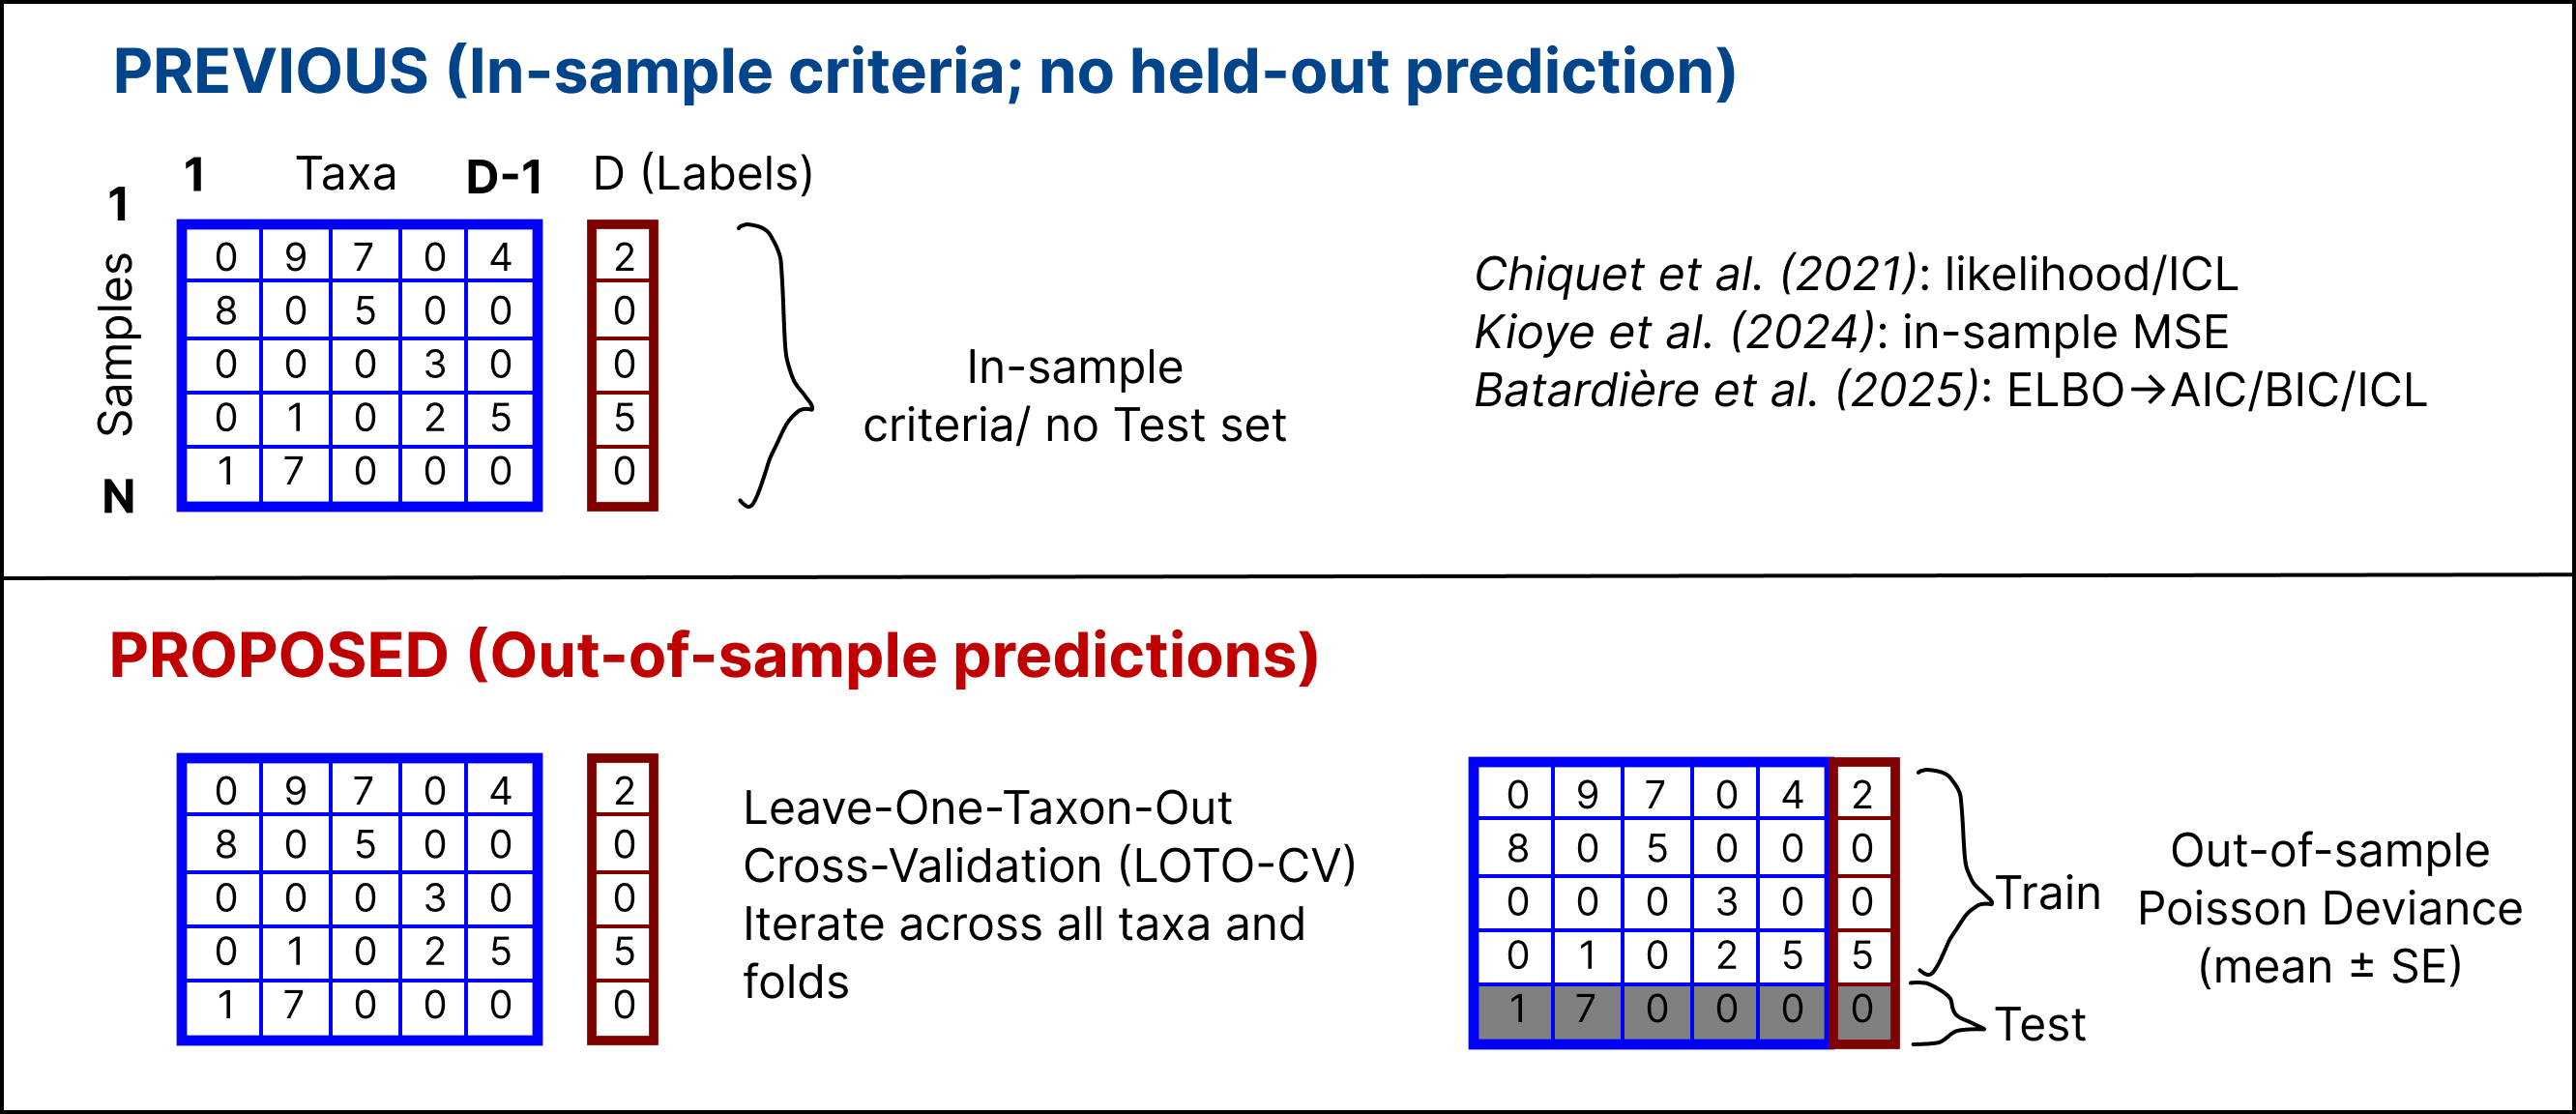
\includegraphics[width=0.92\textwidth]{figure1_conceptual_protocol}
\caption{Conceptual contrast between earlier evaluation practice and the count-prediction protocol used in this study.
Previous work often assessed count models with in-sample fit criteria computed on the observed abundance matrix.
Our benchmark instead withholds a target taxon, predicts its counts out of sample from the remaining taxa, and scores those predictions with held-out Poisson deviance under leave-one-taxon-out cross-validation.}
\label{fig:pipeline}
\end{figure}

\section{Methods}
\subsection{Datasets}
\subsubsection{Count-prediction datasets}
\label{subsec:count-prediction-datasets}
We evaluated count prediction on a heterogeneous benchmark of 20 microbiome datasets spanning oral, skin, nasal, stool, infant, pediatric, and general gut systems, together with several collections focused on disease including colorectal  (CRC), \textit{Clostridium difficile} infection, HIV, non-alcoholic steatohepatitis, obesity, and type~1 diabetes.
The retained benchmark set includes feature tables at the family, genus, species, and OTU levels and covers a broad range of sample sizes and feature dimensions.
Across datasets, the number of samples ranged from $N=32$ to $N=18{,}270$, the number of features ranged from $D=24$ to $D=257$, and the fraction of zero entries in the benchmarked abundance matrices ranged from $30.64\%$ to $93.01\%$.

The goal of this collection is not to represent a single biological system, but to cover the range of settings in which practitioners actually face a choice between a joint latent count model and a faster penalized regression baseline.
Several dataset families are particularly important for that comparison.
American Gut 2~\citep{McDonald2018}, MehtaRS 2018~\citep{Mehta2018}, and MBQC integrated OTUs~\citep{MBQC2017} represent larger and more heterogeneous microbiome surveys, including a very large benchmark-style study in the MBQC collection.
These datasets are useful because they test whether PLN retains an advantage when sample size is no longer the main bottleneck.

Other datasets probe the opposite end of the benchmark.
Lozupone HIV~\citep{Lozupone2013}, RubelMA 2020~\citep{Rubel2020}, and several of the disease-focused stool datasets have relatively small $N$, moderate or large $D$, or both.
These are the settings in which the balance between latent covariance estimation and penalized univariate fitting becomes most visible.
The benchmark also includes multiple colorectal cancer datasets~\citep{Yu2015, Baxter2016, Zeller2014}, early-life gut studies such as Diabimmune Karelia~\citep{Vatanen2016} and ShaoY 2019~\citep{Shao2019}, and targeted disease collections such as Schubert CDI~\citep{Schubert2014}, which together provide repeated examples of related biological questions under different sample sizes, taxonomic resolutions, and sparsity levels.

This diversity is important for interpretation.
The paper's goal is not to identify a single best-performing method on one cohort, but to determine which properties of the count matrix predict when PLN is worth its added complexity.
The broad spread of $N$, $D$, sparsity, and biological settings is therefore a deliberate part of the benchmark design rather than background variation to be averaged away.

Full dataset metadata, including the representative inventory previously shown in the main manuscript, are provided in Table~S1 of the Supplementary Material.
Full benchmark identifiers and provenance are preserved in the repository metadata for exact reproducibility.


\subsubsection{Network-inference datasets}
\label{subsubsec:network-inference-datasets}
We evaluated network inference on five real microbial interaction benchmarks with experimentally supported edge truth.
These datasets were chosen because each provides an external experimental source of interaction truth rather than a simulated or statistically constructed target.
They therefore allow direct evaluation of edge recovery on biological systems for which pairwise competition, facilitation, or conditional effects were measured independently of the fitted models.

The benchmark contains two distinct kinds of truth.
The first kind targets broad undirected edge recovery.
OMM12~\citep{Weiss2022OMM12} and OMM12 keystone 2023~\citep{Weiss2023Keystone} are defined human gut communities in which community composition was perturbed through coculture, deletion, or keystone-style experiments.
These datasets are well suited to evaluating recovery of an overall community interaction graph because the truth reflects system-wide effects across a small, fully enumerated set of taxa.
PairInteraX~\citep{Zhu2025PairInteraX} plays a complementary role.
It provides a much larger human gut species panel with experimentally measured pairwise coculture interaction labels, which makes it useful for testing whether the same methods still recover true edges when the number of taxa increases substantially.

The second kind targets local or directional effects.
Butyrate assembly 2021~\citep{Clark2021Butyrate} contains singleton, pair, and larger synthetic gut communities, allowing local effects to be defined from pair-vs-singleton abundance shifts.
Host fitness 2018~\citep{Gould2018HostFitness} is a five-species \textit{Drosophila} gut system in which pair-vs-singleton colony counts were linked to host reproductive fitness.
These two datasets are informative because the underlying signal is closer to ``taxon $a$ affects taxon $b$'' than to a single global undirected graph, and thus test whether nodewise and joint graphical procedures behave differently when the truth is more local.

Across these datasets, sample size ranged from $N=109$ to $N=1449$, feature dimension ranged from $D=5$ to $D=96$, and data sparsity ranged from $21.25\%$ to $66.19\%$.
Processed abundance matrices and truth edge sets were harmonized into a common benchmark format so that PLNNetwork and \texttt{GLMNet(Poisson)} could be evaluated under the same scoring rules despite their different biological origins.
Dataset-level metadata are provided in Table~S2 of the Supplementary Material.



\subsection{Competing methods}
\label{subsec:algorithms}

We used different methods for count prediction and network inference.
Let $Y_{ij}$ denote the observed count for sample $i$ and taxon $j$, and let $s_i$ denote the sequencing-depth offset for sample $i$.
For count prediction, we compared a featureless baseline, \texttt{GLMNet(Poisson)}, and PLN.
For network inference, we compared a diagonal baseline, \texttt{GLMNet(Poisson)} neighbourhood selection, and PLNNetwork.

For count prediction, the featureless baseline predicts each target taxon by the training-set mean
\[
\hat{\mu}_{ij} = \bar{Y}_{\cdot j}.
\]
For network inference, the diagonal baseline predicts an empty graph, that is
\[
\hat{A}_{jk} = 0 \qquad \text{for all } j \neq k.
\]

\texttt{GLMNet(Poisson)} fits a penalized Poisson regression for each target taxon~\citep{Friedman2010}.
For count prediction, we model
\[
Y_{ij} \mid Y_{i,-j} \sim \mathrm{Poisson}(\mu_{ij}),
\qquad
\log \mu_{ij} = \log s_i + \beta_{0j} + \sum_{k \neq j} \beta_{jk}\,\log(1 + Y_{ik}),
\]
with coefficients estimated by minimizing
\[
-\ell_j(\beta_{0j}, \beta_j) + \lambda_j \lVert \beta_j \rVert_1.
\]
This yields a separate sparse Poisson regression for each target taxon and does not estimate a joint latent covariance across taxa.
For network inference, we use nodewise neighbourhood selection~\citep{Meinshausen2006}.
An undirected edge is included when the symmetrized coefficient support is nonzero, that is
\[
\hat{A}_{jk} = \mathbb{1}\!\left\{\max\!\big(|\hat{\beta}_{jk}|, |\hat{\beta}_{kj}|\big) > 0\right\}.
\]

PLN fits a Poisson log-normal model with a latent Gaussian layer~\citep{aitchison1989multivariate,Chiquet2021}.
For each sample,
\[
Y_{ij} \mid Z_i \sim \mathrm{Poisson}\!\left(s_i \exp(\eta_j + Z_{ij})\right),
\qquad
Z_i \sim \mathcal{N}(0, \Sigma).
\]
For count prediction, held-out means are obtained from Gaussian conditioning in the latent layer,
\[
\hat{\mu}_{ij}
=
s_i \exp\!\left(\hat{\eta}_j + \hat{m}_{ij \mid -j} + \tfrac{1}{2}\hat{v}_{j \mid -j}\right),
\]
where $\hat{m}_{ij \mid -j}$ and $\hat{v}_{j \mid -j}$ are the conditional latent mean and variance for taxon $j$ given the observed taxa in sample $i$.
To stabilize these predictions, we applied covariance shrinkage with parameter $\alpha \in \{0.0, 0.1, \ldots, 1.0\}$ by scaling the off-diagonal entries of $\hat{\Sigma}$.

PLNNetwork extends PLN by estimating a sparse precision matrix $\Omega = \Sigma^{-1}$ within the same variational framework~\citep{chiquet2019variational,Chiquet2021}.
Conceptually, the fitted model maximizes a penalized variational objective of the form
\[
\mathrm{ELBO}(\eta, \Omega) - \rho \lVert \Omega \rVert_{1,\mathrm{off}},
\]
so that zero off-diagonal entries of $\Omega$ correspond to absent conditional associations.
For network inference, we initialized PLNNetwork from a full PLN fit, evaluated a matched log-spaced penalty grid from $\rho_{\max}$ to $0.005\,\rho_{\max}$, set diagonal penalization to false, and selected the final graph by EBIC.
The estimated interaction graph is therefore
\[
\hat{A}_{jk} = \mathbb{1}\!\left\{\hat{\Omega}_{jk} \neq 0\right\}.
\]

All PLN-based models were fit with variational inference using the \texttt{PLNmodels} package~\citep{Chiquet2021}.
All penalized Poisson regressions were fit with \texttt{glmnet}~\citep{Friedman2010}.

\subsection{Evaluation protocols}
\label{subsec:evaluation-protocols}

\subsubsection{Count-prediction evaluation}

For count prediction, we used leave-one-taxon-out cross-validation (LOTO-CV).
In each outer fold, one taxon is held out as the prediction target and the remaining taxa serve as predictors; this is repeated for every taxon and the scores are averaged.
The outer CV used 3 folds; the inner CV used 3 folds for hyperparameter selection.
The primary metric is held-out Poisson deviance, defined as
\[
  \mathcal{D}(y, \hat\mu) = 2\sum_{i} \left( y_i \log\frac{y_i}{\hat\mu_i} - (y_i - \hat\mu_i) \right),
\]
where $y_i$ are the observed counts and $\hat\mu_i$ are the predicted means.
We used Poisson deviance rather than RMSE, correlation, or absolute-error criteria because the prediction target is a count and both competing models are fitted under Poisson mean assumptions.
Poisson deviance is a proper scoring rule for count data: it is minimised in expectation by the true conditional mean $\mathbb{E}[Y_i \mid x_i]$, so a model that achieves lower held-out deviance genuinely predicts better rather than simply fitting the training data more closely~\citep{Gneiting2007ProperScoring}.
This property, which in-sample criteria such as ELBO and BIC do not share, is what makes held-out Poisson deviance the principled choice for comparing count models out of sample.
Gaussian-style losses such as RMSE are less appropriate here because they ignore the mean-variance relationship that is central to the comparison.
For \texttt{GLMNet(Poisson)}, the regularization parameter $\lambda$ was selected by inner-fold Poisson deviance using \texttt{cv.glmnet}.
For PLN, the shrinkage parameter $\alpha$ was selected by 3-fold inner cross-validation on Poisson deviance.
The featureless baseline serves as a lower bound: any algorithm with higher deviance than the featureless baseline provides no useful predictive signal.

\subsubsection{Network-inference evaluation}

For network inference, estimated interaction graphs were compared against experimentally validated microbial interactions from five ground-truth datasets: PairInteraX~\citep{Zhu2025PairInteraX}, OMM12~\citep{Weiss2022OMM12}, OMM12 keystone 2023~\citep{Weiss2023Keystone}, butyrate assembly 2021~\citep{Clark2021Butyrate}, and host fitness 2018~\citep{Gould2018HostFitness}.
Each dataset provides experimentally derived pairwise interaction labels obtained from co-culture, dropout, or combinatorial abundance experiments.
The primary metrics are precision, recall, and F1 score on edge recovery, computed by matching predicted edges against the ground-truth interaction set.
For PLNNetwork, the penalty parameter was selected by EBIC on the training data.
For \texttt{GLMNet(Poisson)} neighbourhood selection, $\lambda$ was fixed at \texttt{lambda.1se} from \texttt{cv.glmnet}.
The diagonal baseline, which predicts an empty graph, serves as the trivial reference point.

\subsection{Computational setup}
\label{subsec:computational-setup}

All experiments were run on Northern Arizona University's Monsoon high-performance computing cluster~\citep{Buechler2025MonsoonIntro}.
Prediction and network benchmark jobs were executed as single-core Slurm jobs.
PLN-based learners were additionally run with one Torch thread to avoid conflating algorithmic differences with thread-level speedups.

Runtime and memory scaling were profiled using the \texttt{atime} R package on the Vogtmann et al.\ stool species dataset~\citep{Vogtmann2016CRC}.
For the saved profiling run, the number of taxa $p$ was varied from 10 to 1000 at a fixed sample size of $N=110$, and each configuration was run three times.
We report median wall time and peak memory across those repeated measurements.


\section{Results}
\subsection{Count-prediction results}

The central empirical result is that relative predictive performance varies systematically across datasets rather than favoring a single method.
Figure~\ref{fig:nd_mac_scatter} shows that the sample-to-taxon ratio $N/D$ is the primary determinant of the dataset-level winner: PLN wins in 12 of 14 datasets with $N/D < 5$ and in none of the 6 datasets with $N/D \geq 5$.
PLN tends to win when $N/D$ is small and the average dependence among taxa is strong.
\texttt{GLMNet(Poisson)} tends to win when $N/D$ is large and inter-taxon dependence is weaker.

MAC is the strongest secondary signal and provides a visually intuitive summary of inter-taxon dependence strength.
Among datasets where \texttt{GLMNet(Poisson)} wins despite low $N/D$, CosteaPI~2017 ($N/D = 1.56$, MAC $= 0.055$) has distinctly low MAC, consistent with weak community dependence reducing the benefit of PLN's latent layer.
American Gut~1 ($N/D = 2.28$, MAC $= 0.182$) is an outlier where \texttt{GLMNet(Poisson)} wins despite moderate dependence.
Overdispersion is an additional predictor that further distinguishes settings where PLN's latent Gaussian layer is most beneficial.
This aligns with the structure of the PLN model.
Its latent Gaussian layer is most useful when counts depart substantially from the Poisson assumption and when joint dependence among taxa carries predictive signal.

\begin{figure}[!t]
\centering
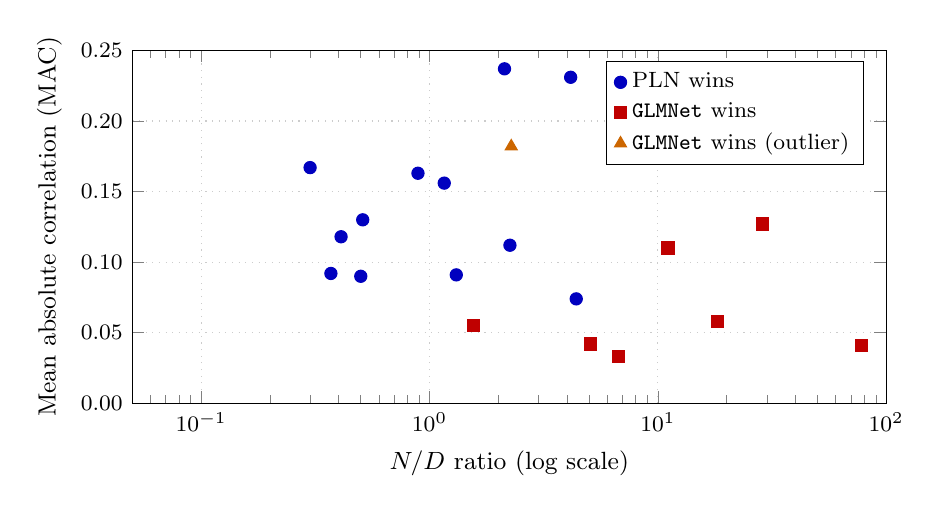
\begin{tikzpicture}
\begin{axis}[
  width=0.92\textwidth,
  height=0.50\textwidth,
  xlabel={$N/D$ ratio (log scale)},
  ylabel={Mean absolute correlation (MAC)},
  xmode=log,
  xmin=0.05, xmax=100,
  ymin=0, ymax=0.25,
  ytick={0, 0.05, 0.10, 0.15, 0.20, 0.25},
  yticklabel style={/pgf/number format/fixed, /pgf/number format/fixed zerofill,
                    /pgf/number format/precision=2, font=\footnotesize},
  ymajorgrids=true,
  xmajorgrids=true,
  grid style={dotted, gray!40},
  tick label style={font=\footnotesize},
  label style={font=\small},
  legend style={font=\footnotesize, at={(0.97,0.97)}, anchor=north east},
  legend cell align=left,
]
\addplot[only marks, mark=*, mark size=2.2pt, blue!75!black]
  coordinates {
    (0.30,0.167)(0.37,0.092)(0.41,0.118)(0.50,0.090)
    (0.51,0.130)(0.89,0.163)(1.16,0.156)(1.31,0.091)
    (2.13,0.237)(2.25,0.112)(4.15,0.231)(4.39,0.074)
  };
\addlegendentry{PLN wins}
\addplot[only marks, mark=square*, mark size=2.2pt, red!75!black]
  coordinates {
    (1.56,0.055)(5.07,0.042)(6.74,0.033)(11.08,0.110)
    (18.30,0.058)(28.80,0.127)(77.74,0.041)
  };
\addlegendentry{\texttt{GLMNet} wins}
\addplot[only marks, mark=triangle*, mark size=2.5pt, orange!80!black]
  coordinates {
    (2.28,0.182)
  };
\addlegendentry{\texttt{GLMNet} wins (outlier)}
\end{axis}
\end{tikzpicture}
\caption{Dataset-level winner as a function of $N/D$ and MAC across the 20-dataset benchmark.
Blue circles: PLN achieves lower held-out Poisson deviance.
Red squares: \texttt{GLMNet(Poisson)} achieves lower held-out Poisson deviance.
The orange triangle marks American Gut~1, a GLMNet win at low $N/D$ and high MAC that runs counter to the general pattern.}
\label{fig:nd_mac_scatter}
\end{figure}

Table~S3 reports the complete retained 20-dataset count-prediction benchmark and highlights the strongest dataset-level contrasts in both directions.
The table includes standard errors, paired $p$-values from a Wilcoxon signed-rank test, and Benjamini--Hochberg adjusted $q$-values to account for multiple testing across the 20 datasets.


\begin{figure}[!t]
  \centering
  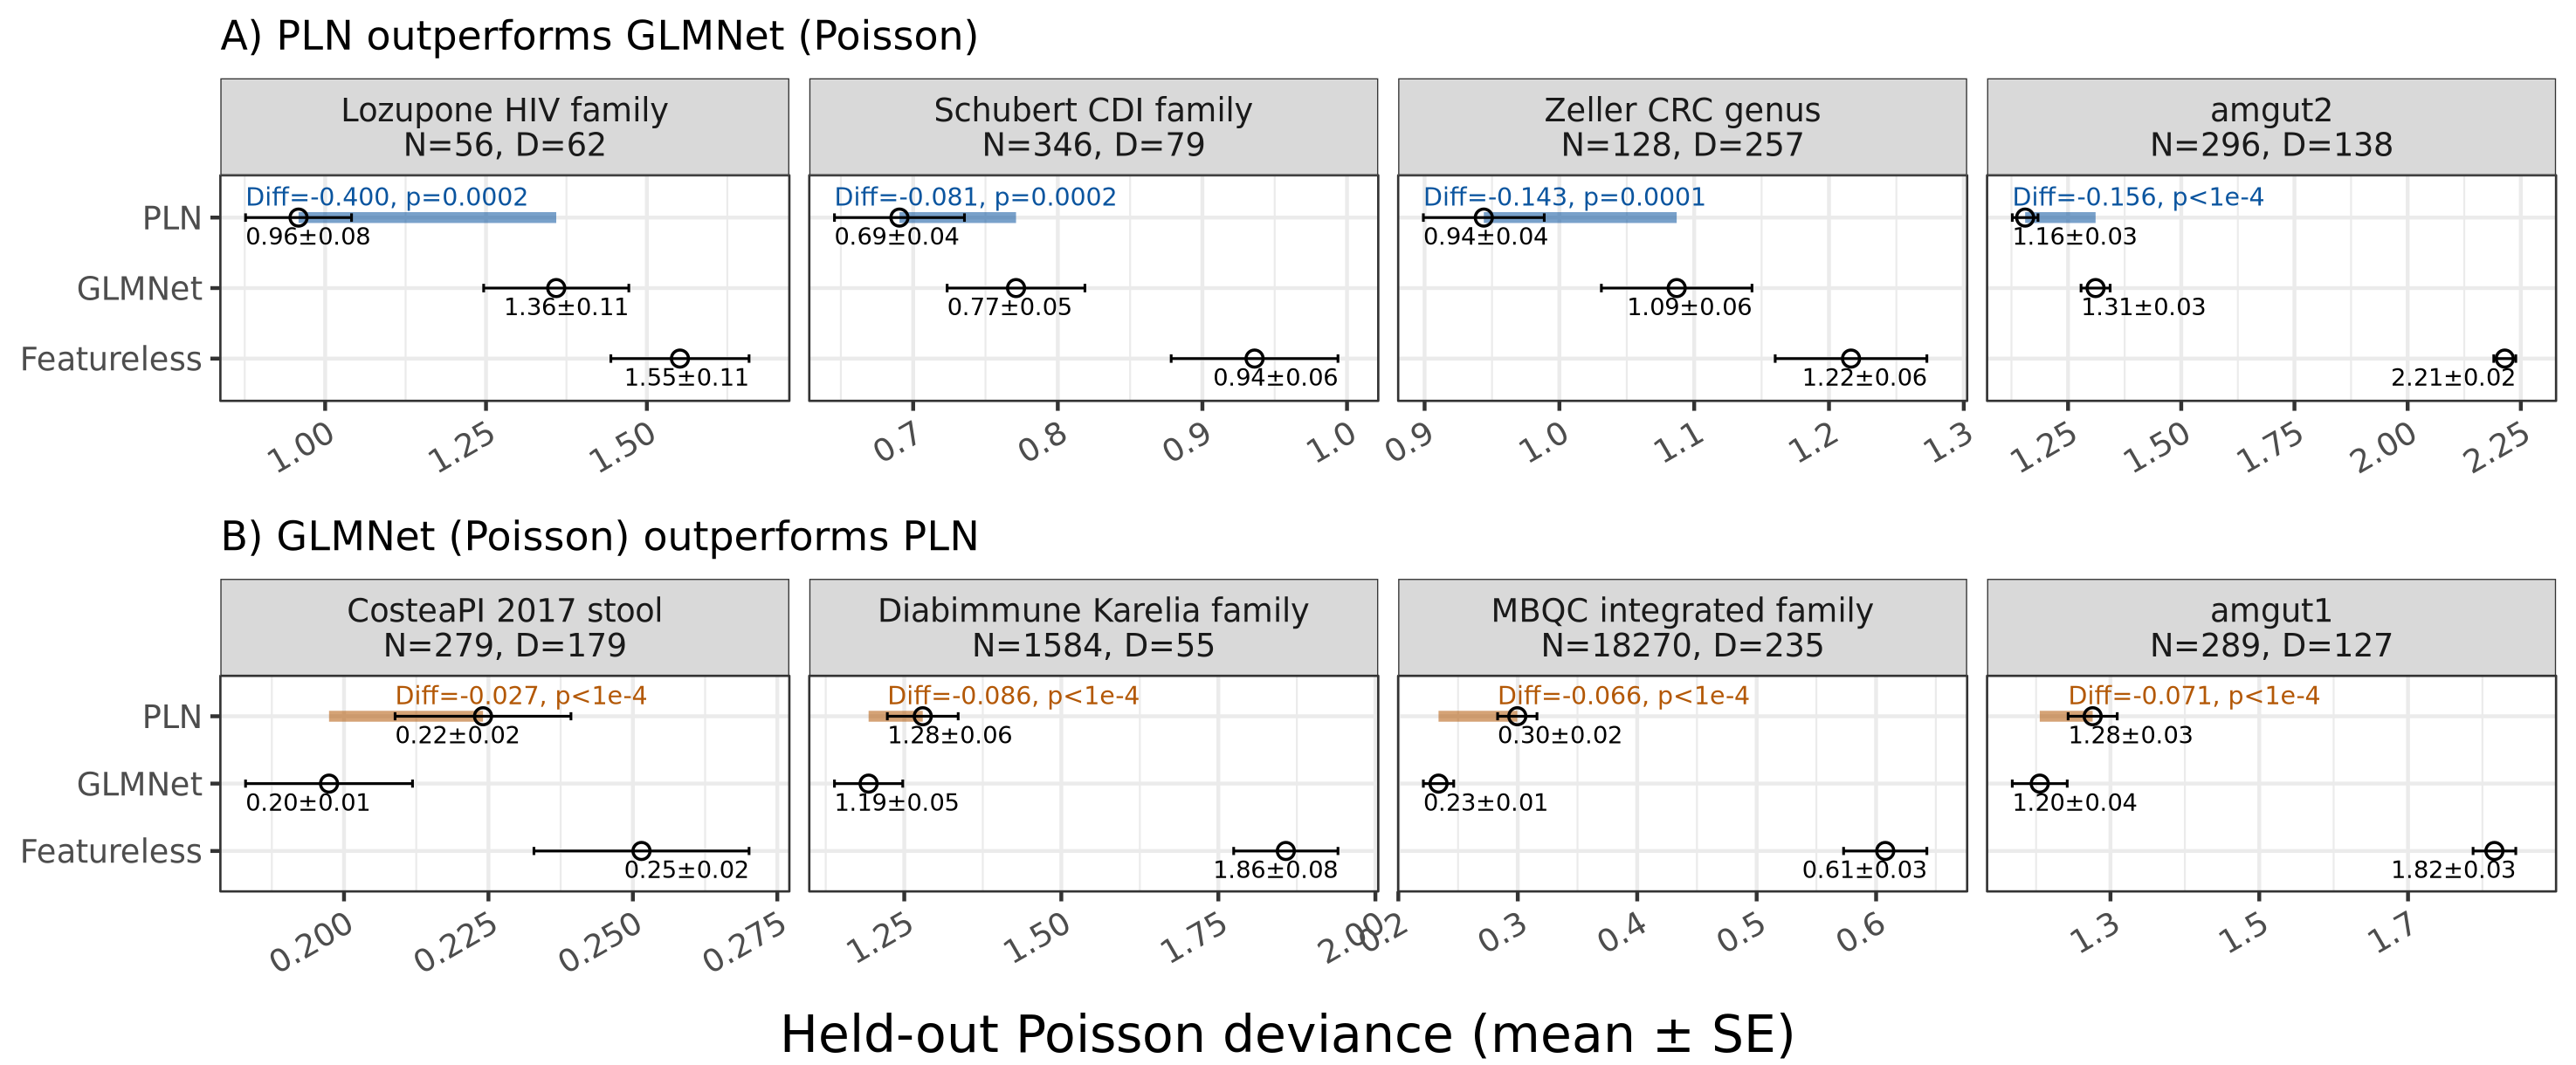
\includegraphics[width=0.95\textwidth]{figure3_count_prediction_case_studies}
  \caption{Representative datasets illustrating both directions of the PLN
  vs.\ GLMNet(Poisson) comparison.
  Top: datasets where PLN achieves lower held-out Poisson deviance.
  Bottom: datasets where GLMNet(Poisson) achieves lower held-out Poisson deviance.
  Each panel reports held-out Poisson deviance (mean $\pm$ SE across three outer
  cross-validation folds) for PLN, GLMNet(Poisson), and the featureless baseline.
  The annotated difference and $p$-value are from the paired comparison of PLN
  and GLMNet(Poisson) across folds.}
  \label{fig:count_pred_case_study}
\end{figure}

Figure~\ref{fig:count_pred_case_study} makes the same contrast concrete with representative case studies from both parts of the benchmark.
In the PLN-favorable panel, Lozupone HIV family, Zeller CRC genus, Schubert CDI family, and amgut2 all show clear reductions in held-out Poisson deviance relative to \texttt{GLMNet(Poisson)}.
These are settings in which limited effective sample size or stronger dependence among taxa makes joint latent modeling useful.

The lower panel shows the opposite pattern.
CosteaPI 2017 stool, MBQC integrated, Diabimmune Karelia, and amgut1 all favor \texttt{GLMNet(Poisson)}, with the largest advantages appearing in better-sampled settings where independent penalized regressions are already sufficient.
In all eight examples, both fitted methods improve over the featureless baseline, indicating that the comparison is between two informative models rather than between signal and noise.


These results suggest a simple practical rule.
PLN is most attractive when $N/D$ is small, inter-taxon dependence is strong, and counts are overdispersed, because those are the settings in which latent covariance estimation appears to improve prediction.
\texttt{GLMNet(Poisson)} becomes preferable as $N/D$ grows and counts approach the Poisson limit, where the extra flexibility of PLN adds cost without commensurate gains.
These are empirical heuristics rather than hard thresholds, but they provide a more concrete starting point for method selection than has previously been available.


\subsection{Network-inference results}
\label{subsec:network-inference-results}


\begin{figure}[!t]
  \centering
  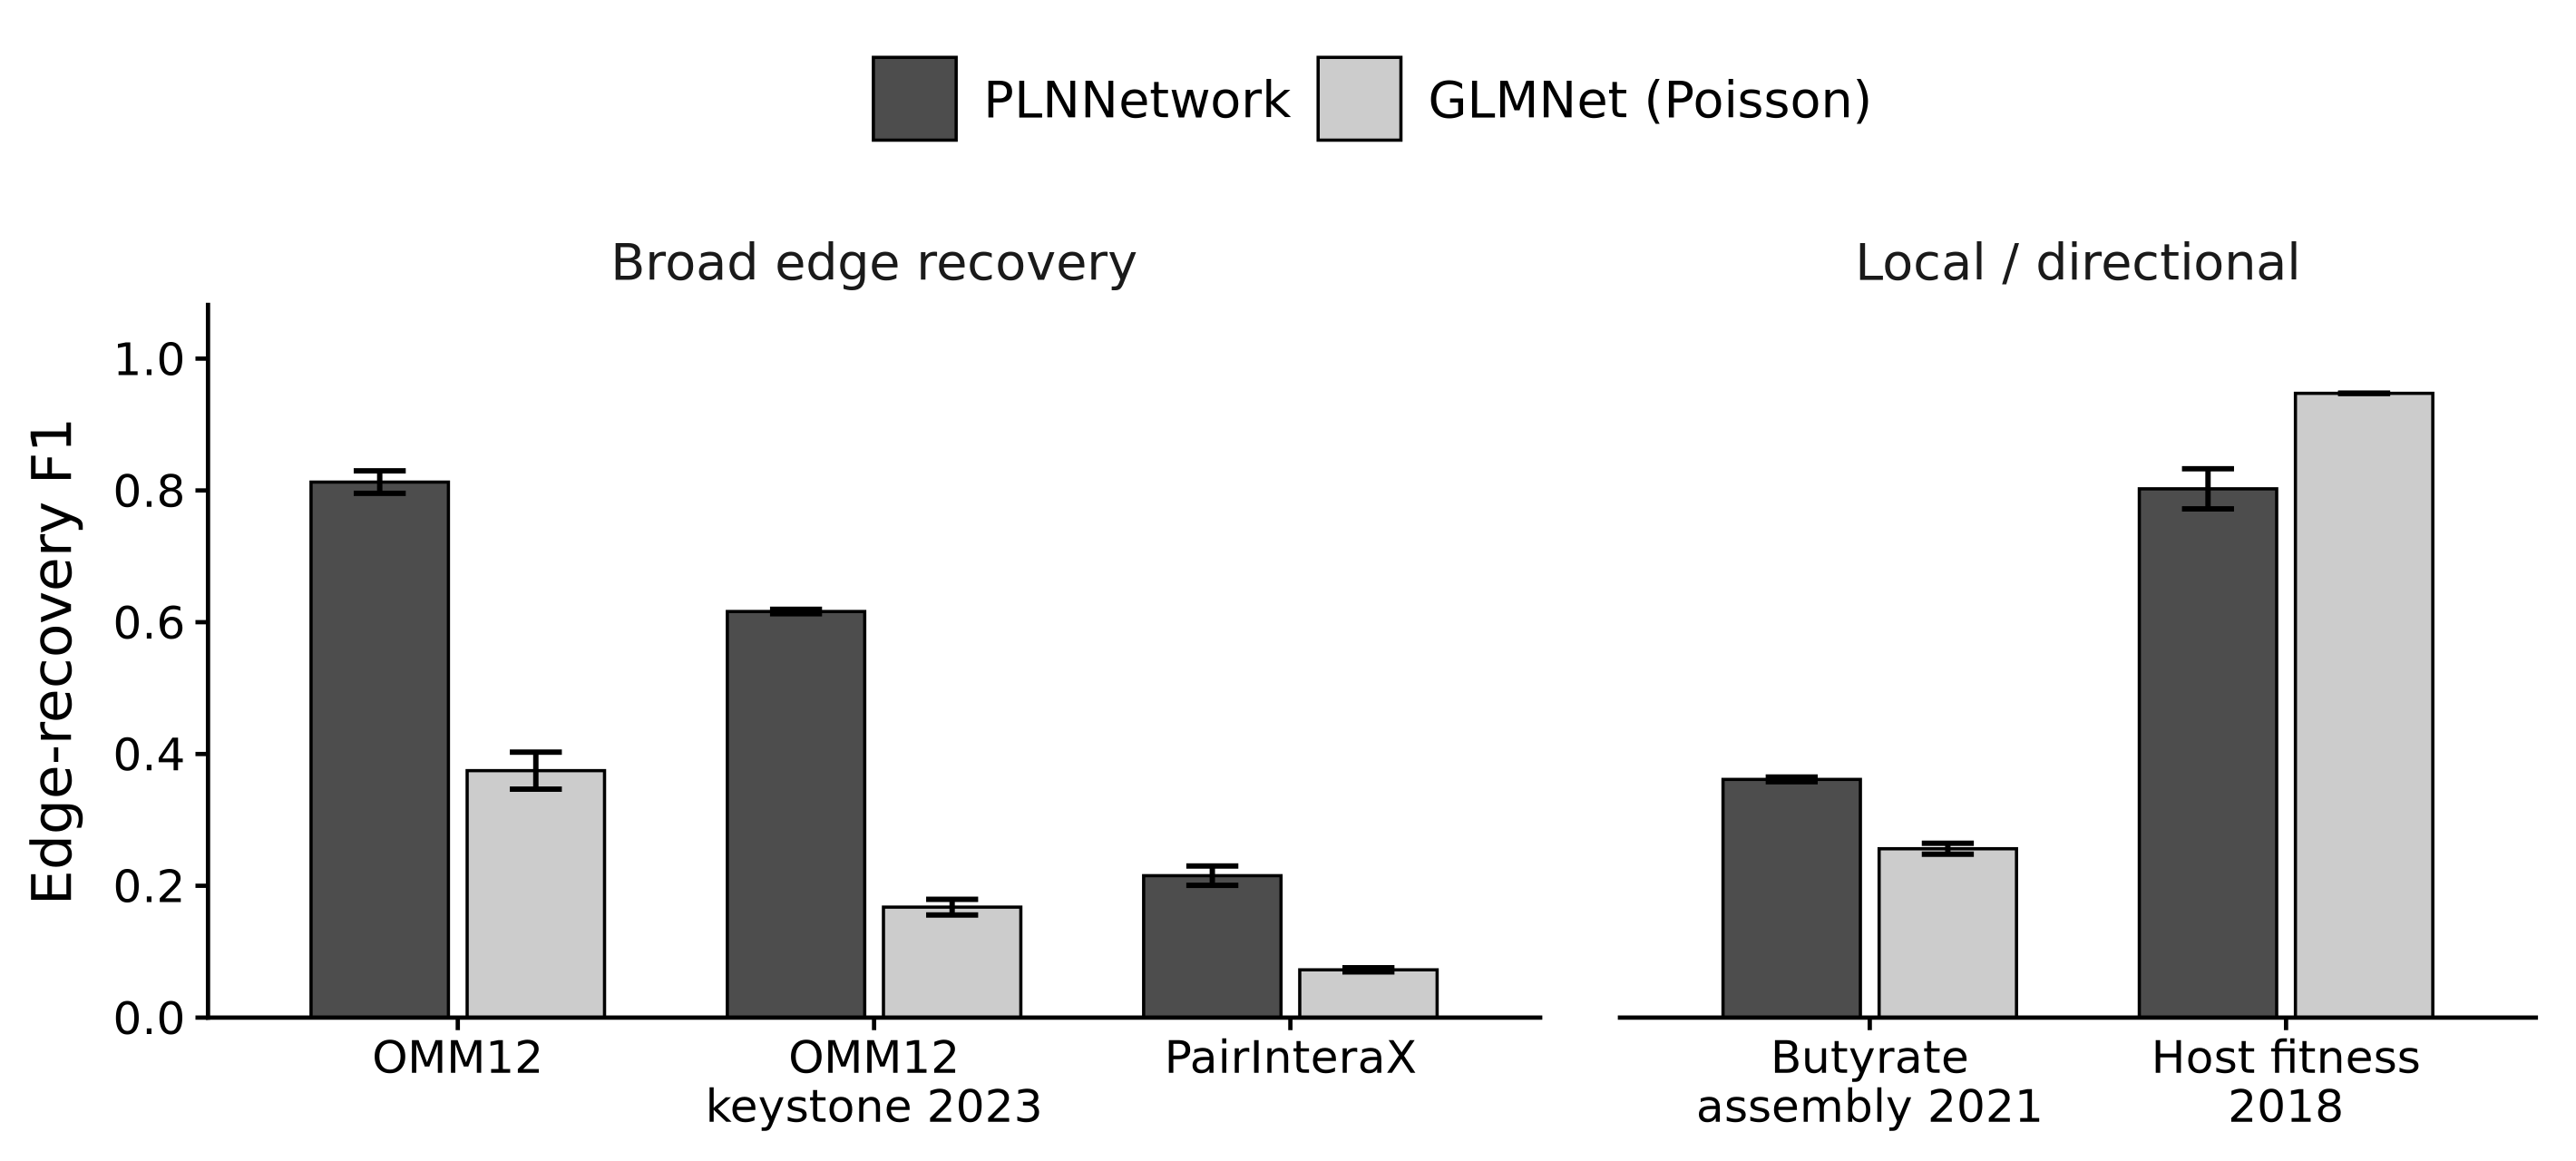
\includegraphics[width=0.94\textwidth]{figure4_network_f1_benchmarks}
  \caption{Edge-recovery F1 on five experimental ground-truth datasets for
  PLNNetwork and \texttt{GLMNet(Poisson)}.
  Datasets are grouped by ground-truth type: broad edge recovery (OMM12,
  OMM12 keystone 2023, PairInteraX) and local/directional (butyrate assembly 2021,
  host fitness 2018).
  Bars show mean F1 over $B = 20$ bootstrap resamples of the abundance matrix;
  error bars are $\pm 1$ SE.}
  \label{fig:network_f1}
\end{figure}

PLNNetwork outperforms \texttt{GLMNet(Poisson)} on four of the five interaction-truth datasets, but the margin depends strongly on the type of biological truth being evaluated (Figure~\ref{fig:network_f1}).
On the three broad edge-recovery datasets, PLNNetwork has the clearer advantage.
Its mean bootstrap F1 exceeds that of \texttt{GLMNet(Poisson)} on OMM12 ($0.81 \pm 0.02$ versus $0.37 \pm 0.03$), OMM12 keystone 2023 ($0.62 \pm 0.003$ versus $0.17 \pm 0.01$), and PairInteraX ($0.22 \pm 0.01$ versus $0.07 \pm 0.003$).
These datasets reward recovery of a global undirected interaction structure, which matches the inductive bias of a sparse latent precision matrix.

The OMM12 example in Figure~\ref{fig:network_case_omm12} illustrates this contrast.
OMM12 is a defined synthetic gut community comprising twelve bacterial taxa: \textit{Enterococcus faecalis} (KB1), \textit{Bifidobacterium animalis} (YL2), \textit{Acutalibacter muris} (KB18), \textit{Muribaculum intestinale} (YL27), \textit{Flavonifractor plautii} (YL31), \textit{Enterocloster clostridioformis} (YL32), \textit{Akkermansia muciniphila} (YL44), \textit{Turicimonas muris} (YL45), \textit{Clostridium innocuum} (I46), \textit{Bacteroides caecimuris} (I48), \textit{Limosilactobacillus reuteri} (I49), and \textit{Blautia coccoides} (YL58).
The experimental graph is relatively dense and dominated by negative interactions.
PLNNetwork recovers much of that structure, whereas \texttt{GLMNet(Poisson)} returns a substantially sparser graph with a different balance of edge signs.

The local and directional datasets tell a more nuanced story.
On butyrate assembly 2021, PLNNetwork retains a modest advantage ($0.36 \pm 0.004$ versus $0.26 \pm 0.008$).
On host fitness 2018, however, the ranking reverses and \texttt{GLMNet(Poisson)} achieves the best overall recovery ($0.95 \pm 0.00$ versus $0.80 \pm 0.03$).
This contrast is shown in Figure~S1 of the Supplementary Material.
The five taxa are \textit{Lactobacillus plantarum} (LP), \textit{Lactobacillus brevis} (LB), \textit{Acetobacter pasteurianus} (AP), \textit{Acetobacter tropicalis} (AT), and \textit{Acetobacter orientalis} (AO).
PLNNetwork recovers part of the experimentally supported structure but misses edges involving AO and introduces a positive LP--LB edge that is not present in the truth.
By contrast, \texttt{GLMNet(Poisson)} closely matches the local negative interaction pattern and misses only one true edge.
In this setting, the ground truth is driven by targeted pairwise effects rather than by a broad undirected community network, and nodewise Poisson regressions appear better aligned with that local signal.

\begin{figure}[!t]
  \centering
  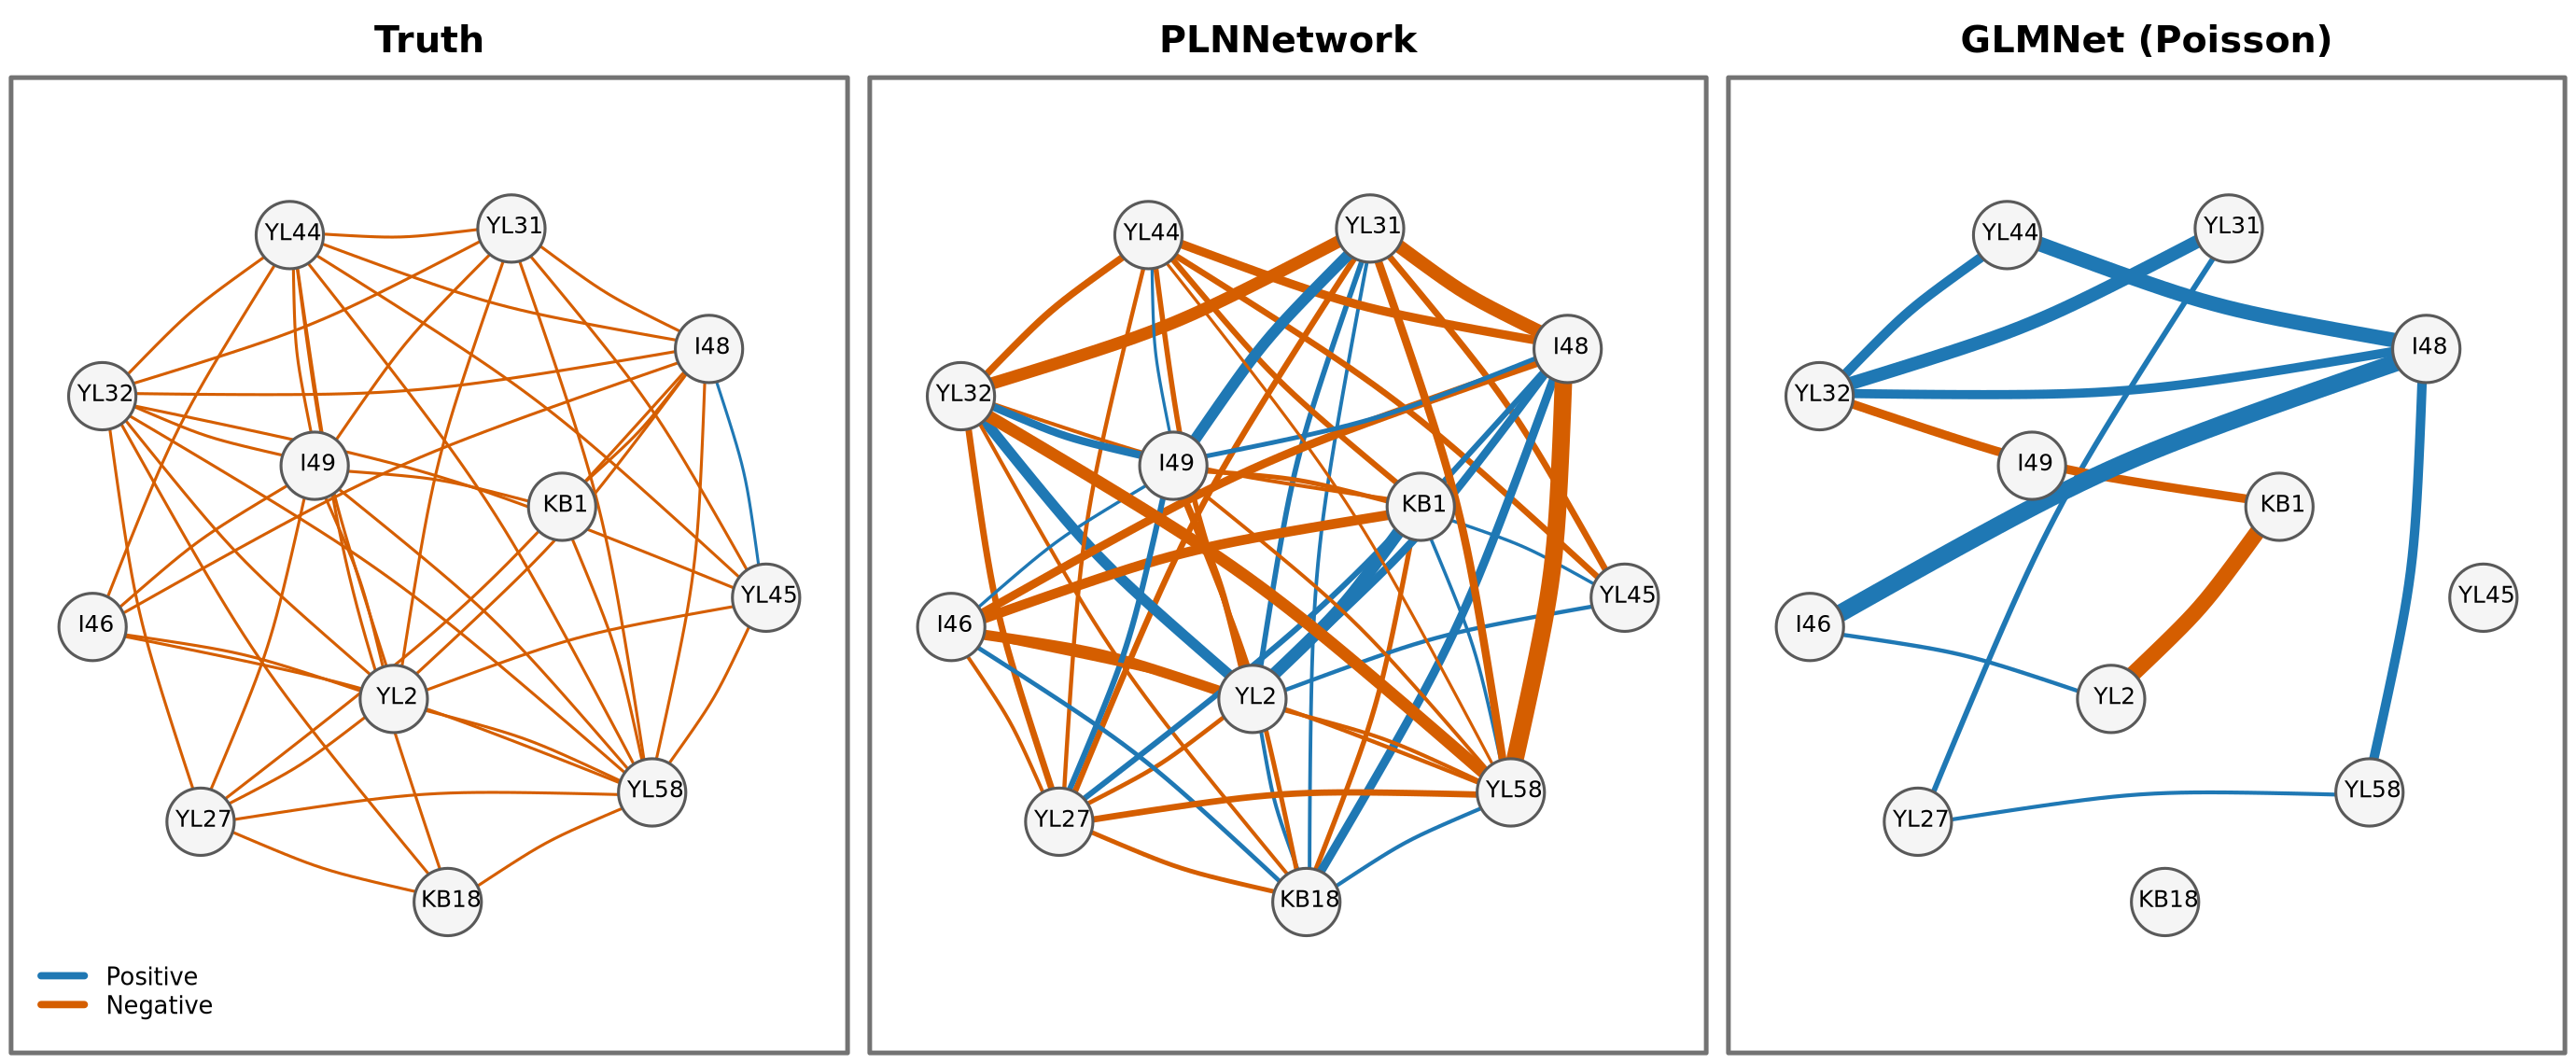
\includegraphics[width=0.94\textwidth]{figure5_omm12_network_comparison}
  \caption{Ground-truth and inferred networks for the OMM12 defined community (12 taxa).
  Each panel shows the experimental ground truth (left), the PLNNetwork prediction
  (centre), and the \texttt{GLMNet(Poisson)} prediction (right).
  Node labels are strain codes: KB1 (\textit{E.\ faecalis}), YL2 (\textit{B.\ animalis}), KB18 (\textit{A.\ muris}), YL27 (\textit{M.\ intestinale}), YL31 (\textit{F.\ plautii}), YL32 (\textit{E.\ clostridioformis}), YL44 (\textit{A.\ muciniphila}), YL45 (\textit{T.\ muris}), I46 (\textit{C.\ innocuum}), I48 (\textit{B.\ caecimuris}), I49 (\textit{L.\ reuteri}), YL58 (\textit{B.\ coccoides}).
  Edge colour indicates interaction sign (blue: positive, orange: negative).}
  \label{fig:network_case_omm12}
\end{figure}

\subsection{Computational scaling}
\label{subsec:computational-scaling}

\begin{figure}[!t]
  \centering
  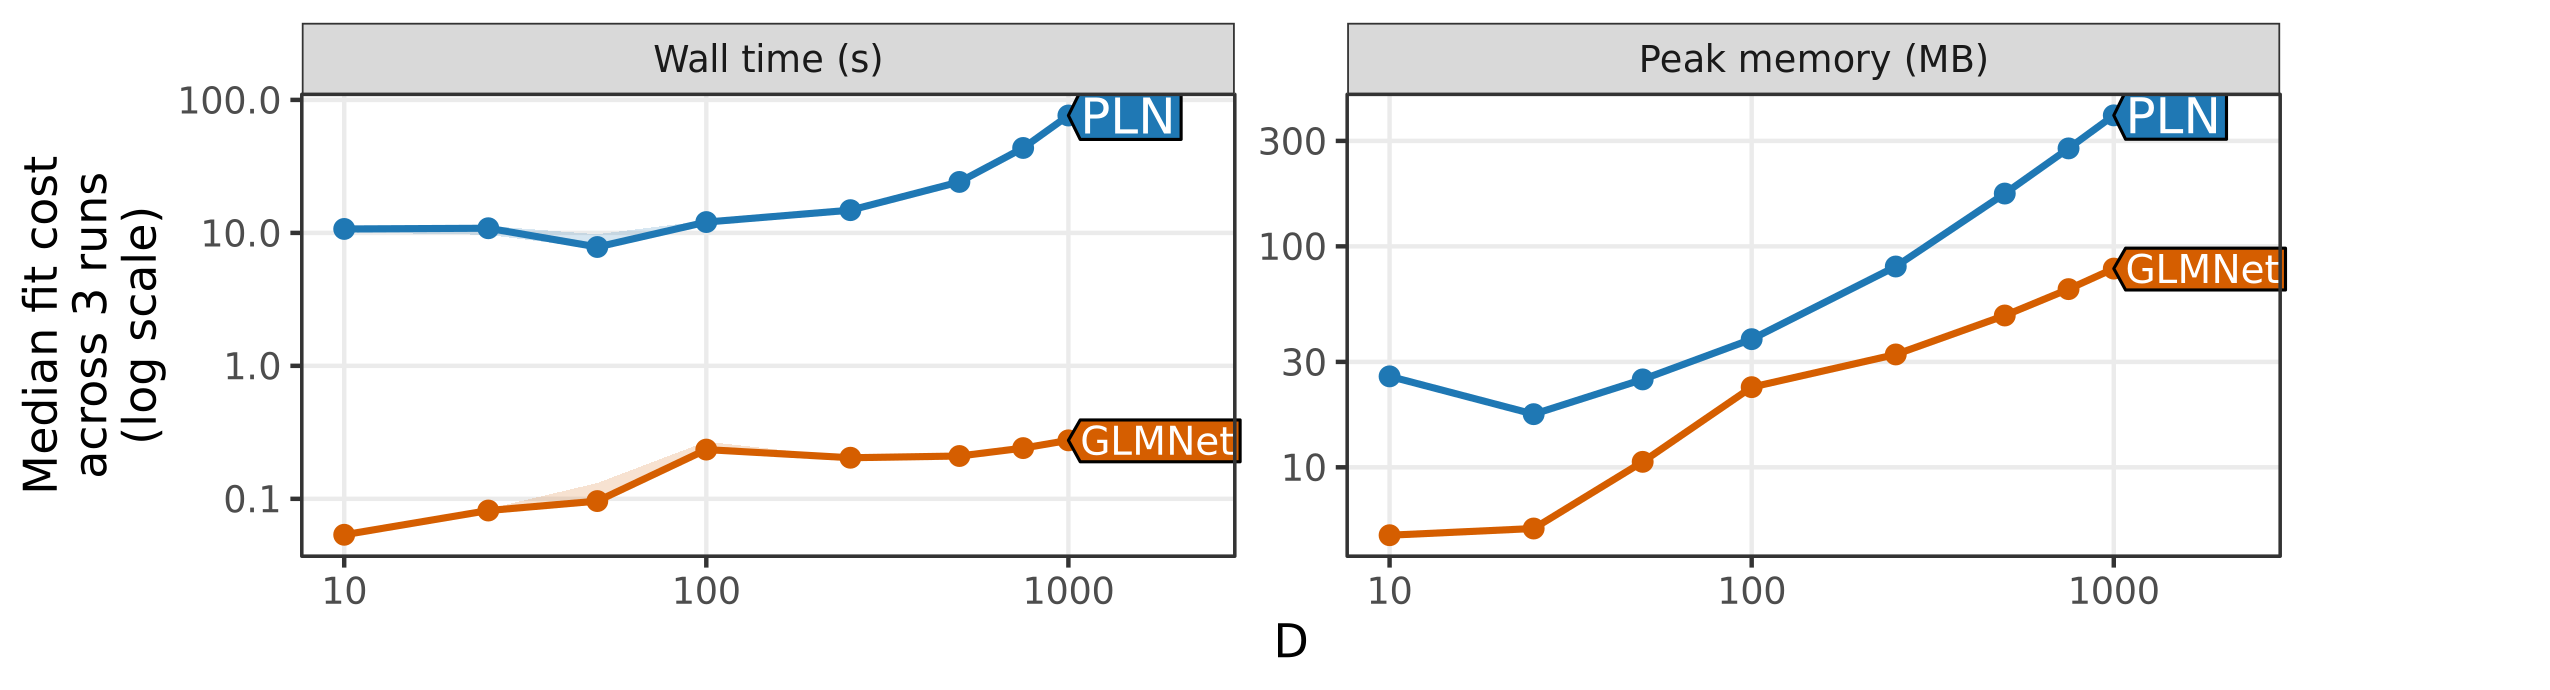
\includegraphics[width=0.94\textwidth]{figure6_computational_scaling}
  \caption{Median wall time (left) and peak memory (right) as a function of the
  number of taxa $D$, profiled on the Vogtmann et al.\ stool species dataset
  ($N = 110$) using the \texttt{atime} R package.
  Each point is the median of three runs; $D$ ranges from 10 to 1000.
  Both axes are on a log scale.}
  \label{fig:atime}
\end{figure}

Computational cost differs sharply between the two model classes.
Across the full range of $D$ values in Figure~\ref{fig:atime}, PLN is consistently slower and more memory-intensive than \texttt{GLMNet(Poisson)}.
At $D = 1000$, PLN requires about 76\,s of wall time and 392\,MB of peak memory, whereas \texttt{GLMNet(Poisson)} requires about 0.28\,s and 79\,MB.

The scaling pattern matches the model structure.
PLN must estimate and manipulate a dense latent covariance matrix, so its cost increases much more quickly with dimension.
\texttt{GLMNet(Poisson)} fits separate penalized regressions and remains comparatively cheap even at the largest tested dimension.
Even so, the observed PLN costs remain manageable on the benchmark sizes studied here, which makes the practical trade-off one of speed versus accuracy rather than feasibility versus infeasibility.


\section{Discussion}
\label{sec:discussion}

The count-prediction results have a clear statistical interpretation.
PLN must estimate a latent covariance structure with $O(D^2)$ degrees of freedom, so its advantage depends on whether the data contain enough information to support that extra layer.
When $N/D$ is small, inter-taxon dependence is strong, and counts are overdispersed, the latent Gaussian component captures signal that independent Poisson regressions miss.
When $N/D$ is large or inter-taxon dependence is weak, the extra flexibility of PLN adds variance and computational cost without improving prediction.
The win-rate pattern is direct: PLN takes 12 of 14 datasets below $N/D = 5$ and zero of the 6 above it, with MAC and overdispersion providing additional explanatory power for the residual cases.

The datasets where PLN shows the strongest gains illustrate the biological context.
Castro-Nallar~2015 (oral cavity, $N/D = 0.30$, $+27\%$) and Lozupone~HIV ($N/D = 0.89$, $+30\%$) are small clinical studies from body sites and disease states known for tight bacterial co-associations, where the joint latent structure captures signal that independent regressions miss.
Baker~NASH/obesity ($N/D = 1.16$, $+30\%$) and Ross~obesity ($N/D = 0.51$, $+30\%$) involve metabolically disrupted gut communities where co-abundance patterns among taxa are elevated.
By contrast, PLN's largest losses occur in large population surveys: MBQC ($N/D = 77.74$, $-28\%$) and MehtaRS~2018 ($N/D = 5.07$, $-25\%$) are high-throughput multi-site collections where samples are abundant relative to taxa and the benefit of modeling joint dependence vanishes.
This suggests PLN is most valuable when studying disrupted or anatomically distinct communities under resource-constrained sampling, and that \texttt{GLMNet(Poisson)} suffices when large healthy cohorts are available.

The network-inference results point to a similar match between model structure and evaluation target.
PLNNetwork estimates a sparse undirected precision matrix and therefore aligns naturally with broad community-level interaction structure.
\texttt{GLMNet(Poisson)} uses nodewise regressions and is correspondingly better suited to local or directional effects.
The host fitness benchmark is the clearest example of this distinction, because its truth labels reflect targeted pairwise effects rather than a single global undirected graph.

Several limitations should be kept in mind.
The 20 count-prediction datasets are not fully independent: the benchmark includes multiple colorectal cancer cohorts and multiple HMP body-site collections, so the effective number of independent biological comparisons is somewhat less than 20.
The win-rate pattern is nonetheless consistent across biological contexts, which limits the concern, but the findings should not be interpreted as arising from 20 entirely unrelated experiments.
The comparison is restricted to the Poisson model family by design; SPIEC-EASI~\citep{Kurtz2015SPIECEASI} and SparCC~\citep{Friedman2012SparCC} operate under compositional log-ratio assumptions that differ fundamentally from the Poisson likelihood, and including them would conflate model family with evaluation protocol.
The network benchmark uses all five experimental ground-truth datasets with publicly available microbial interaction truth that we are aware of; the scarcity of such data reflects fundamental experimental constraints rather than a selective choice, and the conclusions should be interpreted in light of this limitation.
Both fitted methods also receive the same log1p-transformed inputs, a design choice that improves comparability but may not be optimal for PLN.
Finally, the computational profiling is based on a single dataset and single-core execution, so it should be interpreted as a controlled comparison rather than as an exhaustive systems benchmark.

\section{Conclusion}
\label{sec:conclusion}

This study provides a systematic empirical comparison of PLN and penalized Poisson regression for microbiome count prediction and interaction recovery.
Across 20 real count datasets and five interaction-truth benchmarks, neither model class dominates universally.
For count prediction, PLN is most useful when samples are scarce relative to dimension and counts are strongly overdispersed.
\texttt{GLMNet(Poisson)} becomes the better practical choice as $N/D$ grows and the data become closer to the Poisson setting.
For network inference, PLNNetwork is stronger on broad undirected community graphs, whereas \texttt{GLMNet(Poisson)} is better matched to local or directional effects.
Although PLN is substantially more expensive computationally, its observed costs remain practical on the benchmark sizes studied here.
These results give practitioners concrete guidance for deciding when latent dependence modeling is likely to justify its added complexity.

\paragraph{Key findings.}
The benchmark yields four main observations.
First, $N/D$ is the strongest predictor of the count-prediction winner.
Second, MAC is the strongest secondary signal: datasets with high inter-taxon dependence tend to favor PLN even after accounting for $N/D$.
Third, overdispersion provides additional discriminative power beyond $N/D$ and MAC, consistent with PLN's latent Gaussian layer being most beneficial when counts depart substantially from the Poisson assumption.
Third, the network results depend on the kind of biological truth being evaluated, with PLNNetwork favored by broad undirected structure and \texttt{GLMNet(Poisson)} favored by local or directional effects.
Fourth, PLN is substantially more expensive than \texttt{GLMNet(Poisson)}, but the observed costs remain manageable for contemporary microbiome benchmark sizes.

\paragraph{Future directions.}
Several directions follow from the limitations of this study.
First, the benchmark draws from a finite set of public datasets; broader coverage of environments such as soil, marine, and host-associated systems, as well as diverse sequencing protocols, would strengthen the generalisability of the conclusions.
Second, all algorithms received the same \texttt{log1p}-transformed input~\citep{doi:10.1128/mSystems.00016-19}; different normalisation or offset strategies may shift relative performance, and evaluating PLN on raw counts (the input it is designed for) is an important next step.
Third, the comparison is restricted to algorithms in the Poisson family; extending the protocol to negative-binomial and zero-inflated models would give a more complete picture of the count-modelling landscape~\citep{10.1038/s41598-024-76513-8,10.1101/538579,10.1093/bioadv/vbae167,Champion2024OneNet}.
Fourth, lightweight diagnostics that estimate recoverable latent dependence (for example, through stability of conditional correlations across folds) could help practitioners decide when PLN is likely to provide benefits before incurring its full computational cost.
Finally, the computational experiments were conducted on Northern Arizona University's Monsoon supercomputer~\citep{Buechler2025MonsoonIntro}; profiling PLN under multi-threaded execution and at larger sample sizes would give a more complete picture of its practical scalability.

\section*{Declarations}

\subsection*{Ethics approval and consent to participate}
Not applicable.

\subsection*{Consent for publication}
Not applicable.

\subsection*{Availability of data and materials}
The datasets analysed in this study are publicly available; accession details and references are provided in Web Table~1.
The benchmark code is available at \url{https://github.com/EngineerDanny/pln_eval}.

\subsection*{Competing interests}
The authors declare that they have no competing interests.

\subsection*{Funding}
This work was supported by the National Science Foundation grant \#2125088 (Rules of Life Program).

\subsection*{Authors' contributions}
DA conceived the study, implemented the benchmark pipeline, performed the analyses, and drafted the manuscript.
TDH advised on methodology, algorithm design, and manuscript revisions.
All authors read and approved the final manuscript.

\subsection*{Acknowledgments}
Computational work was performed on Northern Arizona University's Monsoon high-performance computing cluster~\citep{Buechler2025MonsoonIntro}.

\subsection*{Authors' information}
Not applicable.

\bibliographystyle{plainnat}
\bibliography{references}

\clearpage
\appendix
\section*{Supplementary Material}
\section*{Web Table 1. Count-prediction dataset inventory}
Datasets are sorted by $N/D$.
$^\dagger$American Gut~1 is an outlier in the count-prediction benchmark (see Web Table~3).
\small
\begin{center}
\begin{tabular}{>{\raggedright\arraybackslash}p{0.24\textwidth}>{\raggedright\arraybackslash}p{0.22\textwidth}>{\raggedright\arraybackslash}p{0.08\textwidth}rrr}
\toprule
Dataset & Human system & Level & $N$ & $D$ & Sparsity (\%) \\
\midrule
Castro-Nallar 2015 & oral & Genus & 32 & 107 & 60.28 \\
ChngKR 2016 & skin & Genus & 78 & 211 & 80.66 \\
HMP 2012 & nasal & Species & 91 & 222 & 92.72 \\
Zeller CRC & stool CRC & Genus & 129 & 257 & 58.29 \\
Ross obesity & gut obesity & Genus & 63 & 123 & 67.05 \\
Lozupone HIV & gut HIV & Family & 55 & 62 & 65.75 \\
Baker NASH/obesity & gut NASH/obesity & Family & 64 & 55 & 56.85 \\
Zhao CRC & stool CRC & Genus & 102 & 78 & --- \\
CosteaPI 2017 & stool enterotypes & Genus & 279 & 179 & 71.73 \\
American Gut 2 & gut citizen science & OTU & 294 & 138 & 34.48 \\
Chan NASH & gut NASH & Family & 54 & 24 & --- \\
American Gut 1$^\dagger$ & gut citizen science & OTU & 289 & 127 & --- \\
Alkanani T1D & gut T1D & Family & 112 & 27 & 66.34 \\
Schubert CDI & stool CDI & Family & 347 & 79 & 79.35 \\
MehtaRS 2018 & gut longitudinal & Genus & 928 & 183 & 75.72 \\
ShaoY 2019 & infant gut & Genus & 1644 & 244 & 93.01 \\
Zeevi obesity & gut glycemic response & Family & 820 & 74 & 74.99 \\
HMP16S v13 & multi-site 16S & Family & 2909 & 159 & 87.20 \\
Diabimmune Karelia & infant gut & Family & 1584 & 55 & 53.36 \\
MBQC integrated OTUs & stool benchmark & Family & 18270 & 235 & 89.46 \\
\bottomrule
\end{tabular}
\end{center}
\normalsize

\section*{Web Table 2. Network-inference dataset metadata}
\small
\begin{center}
\begin{tabular}{>{\raggedright\arraybackslash}p{0.18\textwidth}>{\raggedright\arraybackslash}p{0.18\textwidth}>{\raggedright\arraybackslash}p{0.24\textwidth}rrr}
\toprule
Dataset & System & Truth type & $N$ & $D$ & Data sparsity (\%) \\
\midrule
OMM12 & defined human gut bacterial community & experimental coculture and dropout interactions & 109 & 12 & 21.25 \\
OMM12 keystone 2023 & defined human gut bacterial community & experimental dropout-derived abundance-ratio effects & 228 & 11 & 31.50 \\
PairInteraX & human gut species panel & experimental pairwise co-culture interaction labels & 169 & 96 & 25.86 \\
Butyrate assembly 2021 & defined human gut community & pair-vs-singleton abundance shifts & 537 & 26 & 66.19 \\
Host fitness 2018 & \textit{Drosophila} gut community & pair-vs-singleton CFU shifts & 1449 & 5 & 54.56 \\
\bottomrule
\end{tabular}
\end{center}
\normalsize

\section*{Web Table 3. 20-dataset count-prediction results}
Datasets are sorted by $N/D$.
Blue rows are the four strongest PLN-favorable contrasts; orange rows are the four strongest GLMNet-favorable contrasts.
$^\dagger$American Gut~1 is an outlier: GLMNet wins despite low $N/D$ and relatively high MAC.
\small
\setlength{\tabcolsep}{3pt}
\begin{longtable}{p{0.22\textwidth}rrrrrrp{0.08\textwidth}r}
\toprule
Dataset & $N$ & $D$ & $N/D$ & GLMNet & PLN & $\Delta$ & Winner & MAC \\
\midrule
\endfirsthead
\toprule
Dataset & $N$ & $D$ & $N/D$ & GLMNet & PLN & $\Delta$ & Winner & MAC \\
\midrule
\endhead
Castro-Nallar 2015 & 32 & 107 & 0.30 & 0.4857 & 0.3538 & +27.2\% & PLN & 0.167 \\
ChngKR 2016 & 78 & 211 & 0.37 & 0.2139 & 0.1793 & +16.2\% & PLN & 0.092 \\
\rowcolor{blue!8} HMP 2012 & 91 & 222 & 0.41 & 0.3365 & 0.2075 & +38.3\% & PLN & 0.118 \\
Zeller CRC & 129 & 257 & 0.50 & 1.0870 & 0.9439 & +13.2\% & PLN & 0.090 \\
\rowcolor{blue!8} Ross obesity & 63 & 123 & 0.51 & 1.2938 & 0.9046 & +30.1\% & PLN & 0.130 \\
\rowcolor{blue!8} Lozupone HIV & 55 & 62 & 0.89 & 1.3591 & 0.9587 & +29.5\% & PLN & 0.163 \\
\rowcolor{blue!8} Baker NASH/obesity & 64 & 55 & 1.16 & 1.3292 & 0.9337 & +29.8\% & PLN & 0.156 \\
Zhao CRC & 102 & 78 & 1.31 & 0.7487 & 0.6205 & +17.1\% & PLN & 0.091 \\
\rowcolor{orange!10} CosteaPI 2017 & 279 & 179 & 1.56 & 0.1974 & 0.2241 & $-$13.5\% & GLMNet & 0.055 \\
American Gut 2 & 294 & 138 & 2.13 & 1.3108 & 1.1553 & +11.9\% & PLN & 0.237 \\
Chan NASH & 54 & 24 & 2.25 & 1.5787 & 1.2359 & +21.7\% & PLN & 0.112 \\
American Gut 1$^\dagger$ & 289 & 127 & 2.28 & 1.2049 & 1.2761 & $-$5.9\% & GLMNet & 0.182 \\
Alkanani T1D & 112 & 27 & 4.15 & 1.3291 & 1.0756 & +19.1\% & PLN & 0.231 \\
Schubert CDI & 347 & 79 & 4.39 & 0.7711 & 0.6905 & +10.5\% & PLN & 0.074 \\
\rowcolor{orange!10} MehtaRS 2018 & 928 & 183 & 5.07 & 0.1786 & 0.2225 & $-$24.6\% & GLMNet & 0.042 \\
ShaoY 2019 & 1644 & 244 & 6.74 & 0.1571 & 0.1647 & $-$4.8\% & GLMNet & 0.033 \\
Zeevi obesity & 820 & 74 & 11.08 & 0.5570 & 0.5628 & $-$1.1\% & GLMNet & 0.110 \\
HMP16S v13 & 2909 & 159 & 18.30 & 0.3307 & 0.3347 & $-$1.2\% & GLMNet & 0.058 \\
\rowcolor{orange!10} Diabimmune Karelia & 1584 & 55 & 28.80 & 1.1932 & 1.2794 & $-$7.2\% & GLMNet & 0.127 \\
\rowcolor{orange!10} MBQC integrated OTUs & 18270 & 235 & 77.74 & 0.2337 & 0.2996 & $-$28.2\% & GLMNet & 0.041 \\
\bottomrule
\end{longtable}
\normalsize

\section*{Web Figure 1. Host fitness 2018 network comparison}
\begin{center}

\includegraphics[width=\textwidth]{interaction_network_example_host_fitness_2018_2026-04-01}
\end{center}

\section*{Web Figure 2. Dataset-level winner versus $N/D$ and MAC}
\begin{center}
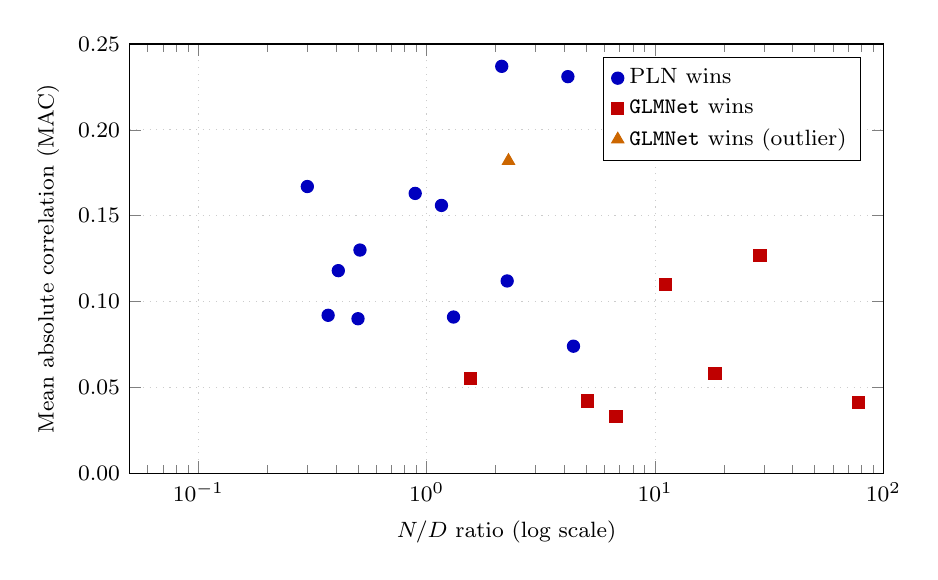
\begin{tikzpicture}
\begin{axis}[
  width=0.92\textwidth,
  height=0.58\textwidth,
  xlabel={$N/D$ ratio (log scale)},
  ylabel={Mean absolute correlation (MAC)},
  xmode=log,
  xmin=0.05, xmax=100,
  ymin=0, ymax=0.25,
  ytick={0, 0.05, 0.10, 0.15, 0.20, 0.25},
  yticklabel style={/pgf/number format/fixed, /pgf/number format/fixed zerofill,
                    /pgf/number format/precision=2, font=\footnotesize},
  ymajorgrids=true,
  xmajorgrids=true,
  grid style={dotted, gray!40},
  tick label style={font=\footnotesize},
  label style={font=\footnotesize},
  legend style={font=\footnotesize, at={(0.97,0.97)}, anchor=north east},
  legend cell align=left,
]
\addplot[only marks, mark=*, mark size=2.2pt, blue!75!black]
  coordinates {
    (0.30,0.167)(0.37,0.092)(0.41,0.118)(0.50,0.090)
    (0.51,0.130)(0.89,0.163)(1.16,0.156)(1.31,0.091)
    (2.13,0.237)(2.25,0.112)(4.15,0.231)(4.39,0.074)
  };
\addlegendentry{PLN wins}
\addplot[only marks, mark=square*, mark size=2.2pt, red!75!black]
  coordinates {
    (1.56,0.055)(5.07,0.042)(6.74,0.033)(11.08,0.110)
    (18.30,0.058)(28.80,0.127)(77.74,0.041)
  };
\addlegendentry{\texttt{GLMNet} wins}
\addplot[only marks, mark=triangle*, mark size=2.5pt, orange!80!black]
  coordinates {
    (2.28,0.182)
  };
\addlegendentry{\texttt{GLMNet} wins (outlier)}
\end{axis}
\end{tikzpicture}
\end{center}

\end{document}
